%!TEX root= ../../../report.tex

\section{From the wheel to the leg} % (fold)
\label{sec:from_the_wheel_to_the_leg}
While the wheel is a young human invention meant to facilitate terrestrial motion, legged locomotion has been the result of millions of years of adaption of the species from the aquatic to a terrestrial field.
During this time, even though other forms of motion on the ground emerged, including limbless or rolling, the tetrapod and quadrupedal motion are the ones that have proved the best performances in terrestrial displacements in terms of relative velocity or jump length, for instance.

\subsection{Discovering the wheel (in robotics)} % (fold)
\label{sub:the_wheel_in_robotics}
Despite the facts above, it was the wheel the mean chosen to implement the ability to move around on the first mobile robots such as Walter's tortoises or the John Hopkins University robot Beast \cite{first_mobile_robot}, \cite{second_mobile_robot}.
This could be explained due to the fact that, as an artificial human creation, the modeling and control of the wheel could be fully mastered during its evolution process, easing its implementation in robotic platforms.
Some examples of this are shown in Figure \ref{fig:mobile_robots}, which depicts three current applications of the wheel in robot platforms.

Although the wheel was chosen as the motion mean to face what can be considered one of the most challenging and unpredictable environment a robot can be subject to, the surface of a new planet, it was not the only option. 
The Space General Corporation firstly studied the use of multi-legged autonomous platforms for lunar exploration in the early 1960's \cite{legged_mot_history1}.
However, their use was eventually discarded due to its poor adaptability due to a too low number of DOF.
The "Spirit" robot in \ref{fig:mobile_rover}, within the NASA's Mars Exploration Rover mission, is the example of the current solution to extraplanetary exploration and a good example of the possibilities and limits entailed by wheel-based locomotion.
It was successfully launched on Mars surface in 2004 and it stayed active and operative until 2010.
However, the end of the mission came from the hand of the terrain. 
A very low-cohesion area of soil made the wheels of the device loose traction and eventually get trapped, preventing from recovering the control of the vehicle and bringing about the end of the mission.

\begin{figure}[h]
\label{fig:mobile_robots}
	\centering
    \begin{subfigure}[b]{0.40\textwidth}
        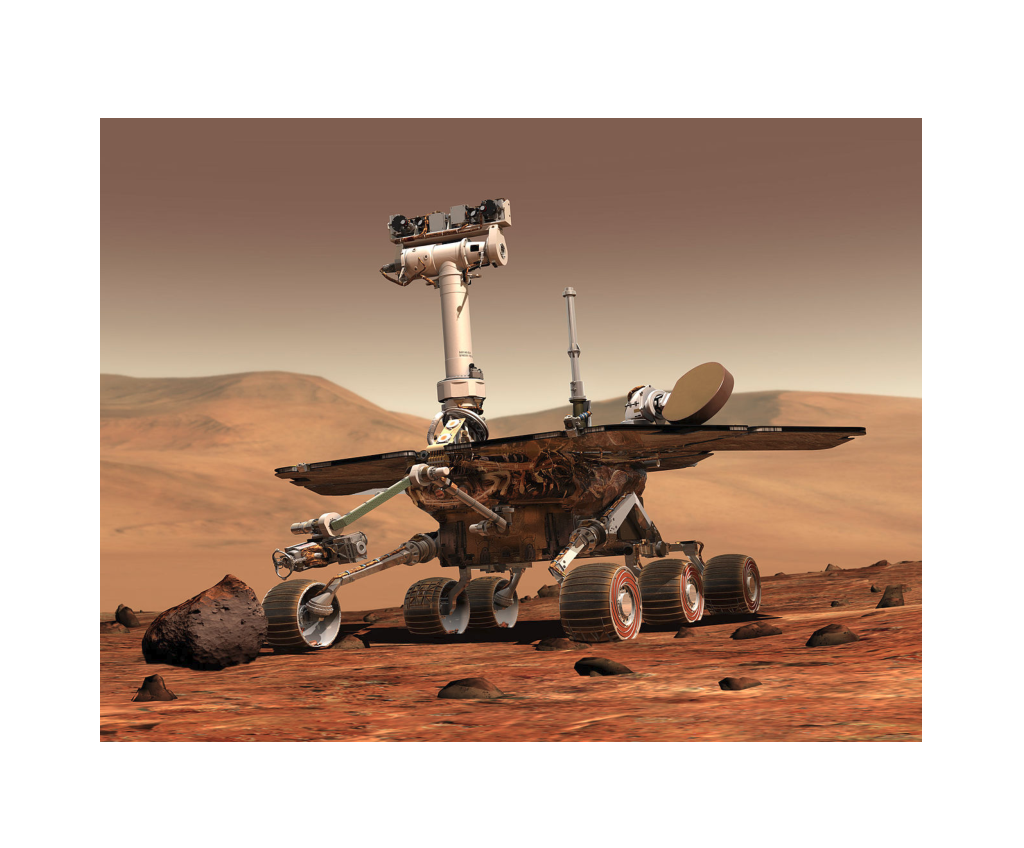
\includegraphics[width=\textwidth]{figures/mobile_rover.pdf}
        \caption{Mars Rover Spirit}
        \label{fig:mobile_rover}
    \end{subfigure}
    \centering
    \begin{subfigure}[b]{0.40\textwidth}
        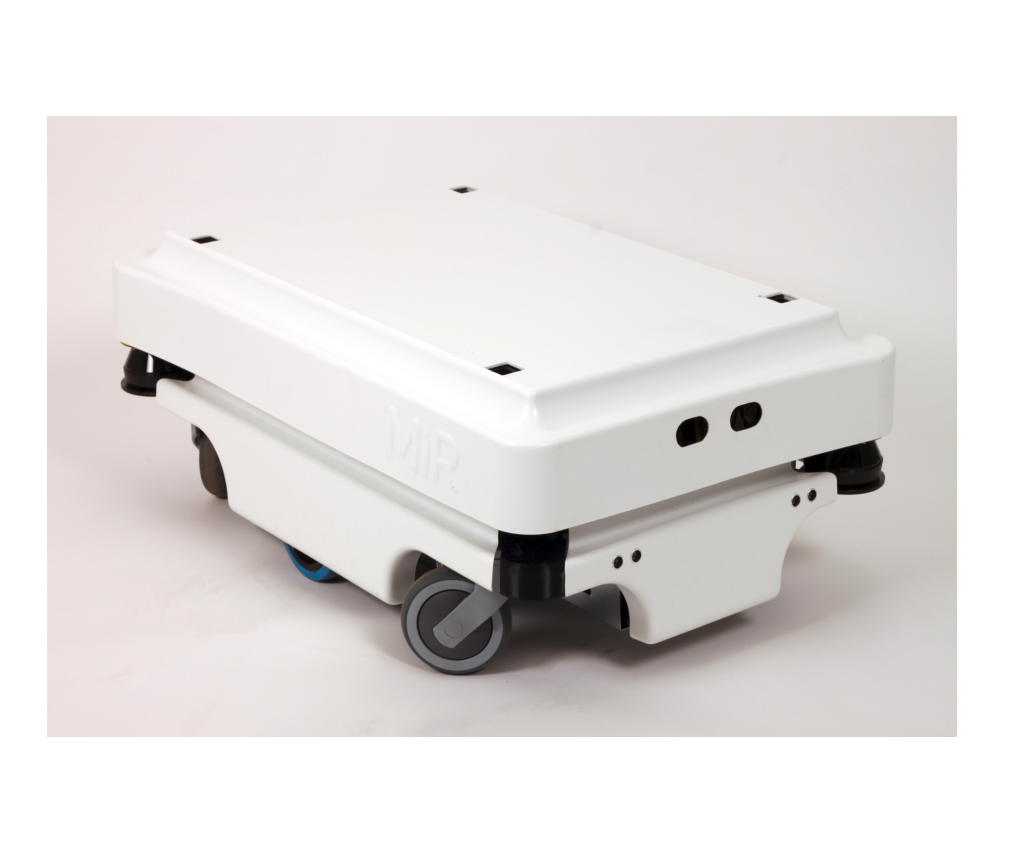
\includegraphics[width=\textwidth]{figures/mobile_mir.pdf}
        \caption{MIR 100 by MIR}
        \label{fig:mobile_mir}
    \end{subfigure}

    \centering
    \begin{subfigure}[b]{0.40\textwidth}
        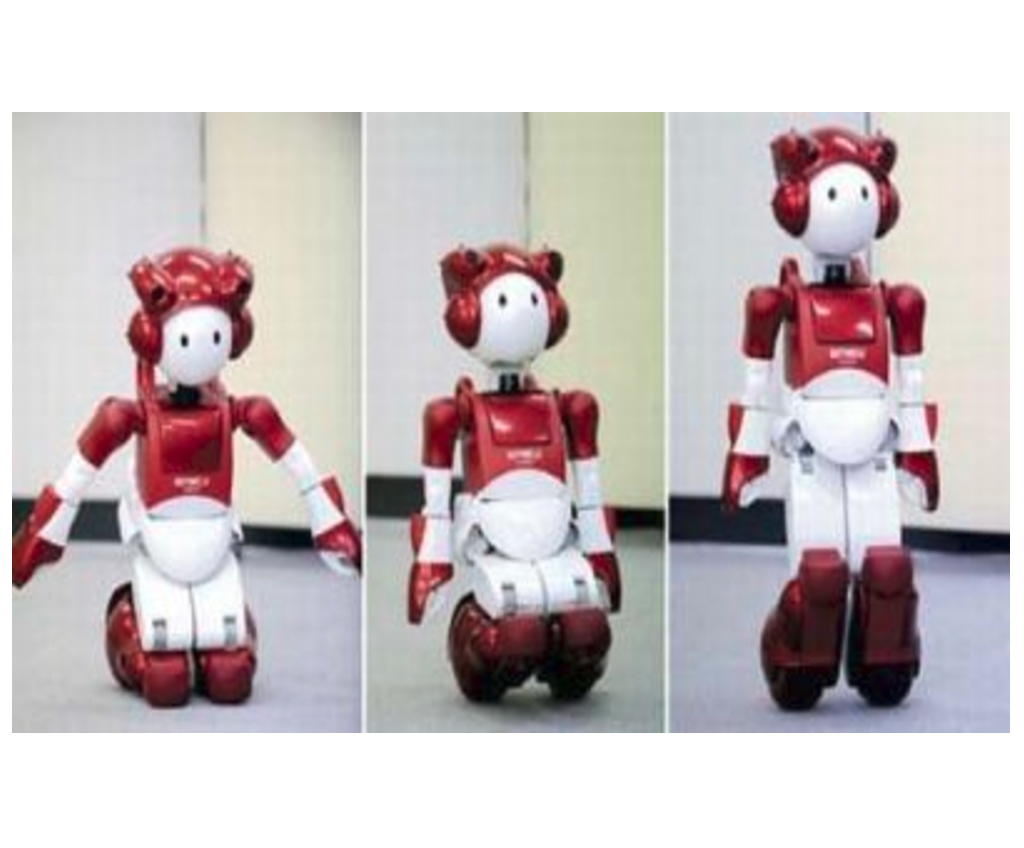
\includegraphics[width=\textwidth]{figures/mobile_hitachi.pdf}
        \caption{EMIEW2, by Hitachi}
        \label{fig:mobile_hitachi}
    \end{subfigure}
\caption{Examples of wheeled robot platform}
\end{figure}

Figure \ref{fig:mobile_mir} shows a MIR 100 robot, a state-of-the-art service robot designed for independent transportation and logistics in a dynamic and unpredictable environment..
As a service robot, it must fulfill strict safety standards and guarantee a secure interaction with users and other equipment while accomplishing its tasks.
Thanks to its wheels configuration, it can achieve an agile mobility, fast reaction capacity and a big load capacity.

\hfill

The EMIEW 2, in \ref{fig:mobile_hitachi}, is an example of midpoint between wheeled and legged locomotion.
Although its motion relies on steering wheels, their placement at the end of two leg-like lower-limbs provides with some of the advantages of bipedal motion, such as active suspension or impact absorption.


% subsection the_wheel_in_robotics (end)

\subsection{Achieving legged motion} % (fold)
\label{sub:legged_motion_in_robotics}
In spite of the great successes attained in the field of wheeled-robotics, possible thanks to the development in engines and the increasing computing capacity of embedded processors, mobile robots based on wheels have not been able to achieve performances in motion comparable to the ones found in nature.
Specially in uneven terrains, velocity, maneuverability, and efficiency are still problems under study.
Besides, the absence of wheels in nature as a result of darwinian evolution ultimately led to questioning \cite{dawkins} if they are truly the best mean to overcome the challenges that displacements in uneven, unknown surfaces yield for robots.
In words of Richard Dawkins \cite{dawkins} "[the wheel] is dependent for maximum efficiency on a prior invention – the road (or other smooth, hard surface)". 
Figure \ref{fig:biped_robots} contains three of the most advanced stages in legged locomotion nowadays.
They have been chosen because they are meaningful current paradigms of what brought about the revolution to the leg-based locomotion systems in the 80's: the conjunction between mechanics and control as the producers of the expected behavior \cite{mit_leg_lab1}.

The STARLeth robot in \ref{fig:starleth}, built at the Autonomous System Lab at ETH, is an example of robot legged robot inspired by nature. 
It is meant at proving that versatility, speed, robustness and efficiency can be achieved together in a legged moving platform \cite{starleth}.
But it also represents the control problems arisen from this kind of locomotion, by definition unstable and complex (12 actuated joints and 6 unactuated DOF). 

In Figure \ref{fig:kaist} the Raptor robot created at KAIST is shown.
This robot is inspired in a velociraptor structure and has been able to achieve a top stable speed on a treadmill of 46 $km/h$, making it the current fastest biped robot (although the Cheetah robot by Boston Dynamics has the record as a quadruped).
However, it is discussed here because of its simple bioinspired design, which combines prosthetic blades with a dynamic tail for stabilization and only required two motors.
This makes it a good illustration of the importance of biomechanics in the overall system.

Finally the ATLAS robot by Boston Dynamics, in \ref{fig:atlas}, represents the state of the art in bipedal autonomous platforms handling unknown, rough terrain and its interaction with dynamically changing environment.
This task for a high degree of freedom mobile manipulator as a humanoid requires a very robust interactive motion planning and control in order to quickly carry out its assignment while overcoming unpredicted situations fast and reliably enough.
The ATLAS is a good illustration of the relevance of a robust but flexible and adaptive control architecture for this kind of machines.


\begin{figure}[h]
\label{fig:biped_robots}
	\centering
    \begin{subfigure}[b]{0.40\textwidth}
        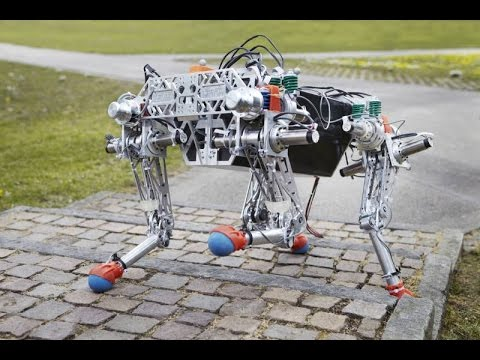
\includegraphics[width=\textwidth]{figures/starleth.jpg}
        \caption{STARLeth}
        \label{fig:starleth}
    \end{subfigure}
    \centering
    \begin{subfigure}[b]{0.40\textwidth}
        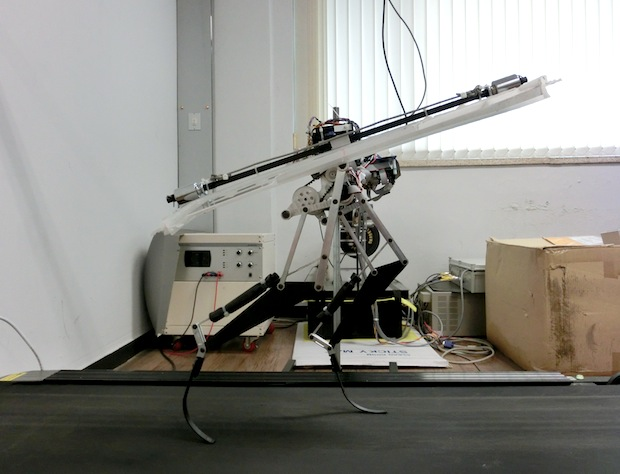
\includegraphics[width=\textwidth]{figures/biped_kaist.jpg}
        \caption{Raptor}
        \label{fig:kaist}
    \end{subfigure}
    \centering


    \begin{subfigure}[b]{0.32\textwidth}
        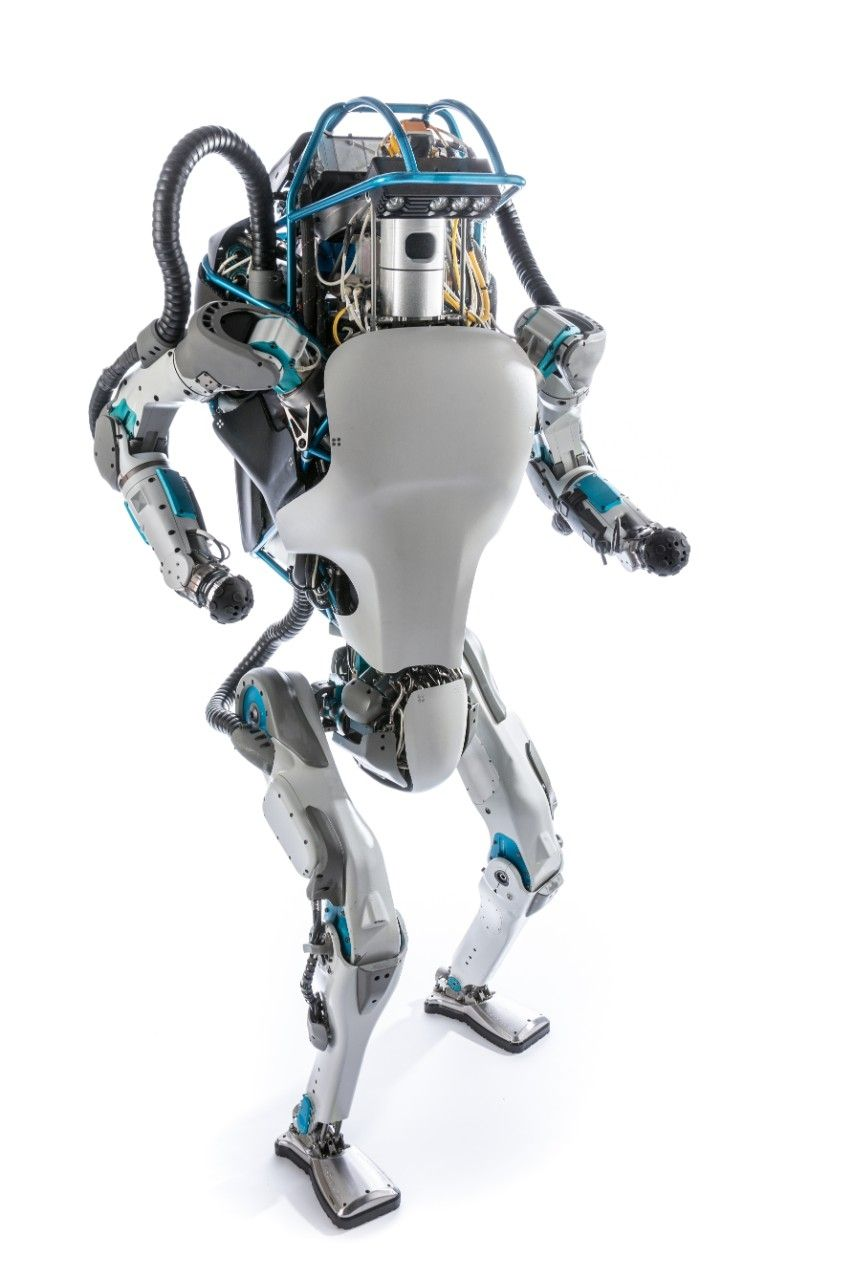
\includegraphics[width=\textwidth]{figures/biped_atlas.jpg}
        \caption{ATLAS}
        \label{fig:atlas}
    \end{subfigure}
    \caption{Examples of legged robot platforms}
\end{figure}


% subsection legged_motion_in_robotics (end)





% section from_the_wheel_to_the_leg (end)